\begin{figure}
\begin{center}
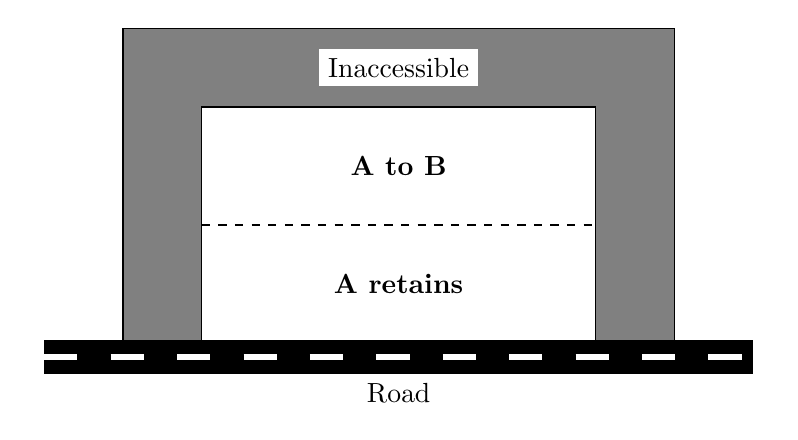
\begin{tikzpicture}
\filldraw[fill=gray]
(0, 0) -- (0, 4) -- (7, 4) -- (7, 0) -- (6, 0)
-- (6, 3) -- (1, 3) -- (1, 0) -- cycle;
\draw[thick, dashed] (1, 1.5) -- (6, 1.5);
\node[fill=white] at (3.5, 3.5) {Inaccessible};
\node at (3.5, 2.25) {\textbf{A to B}};
\node at (3.5, 0.75) {\textbf{A retains}};
\draw[line width=12pt] (-1, -5pt) -- (8, -5pt);
\draw[dash pattern=on 12pt off 12pt, white, line width=2pt]
(-1, -5pt) -- (8, -5pt);
\node[below] at (3.5, -11pt) {Road};
\end{tikzpicture}
\end{center}
\caption{A ``landlocked'' parcel of land.}
\label{f:easements-landlocked}
\end{figure}

An \term{easement by necessity} (or sometimes \term{way by necessity})
arises when land becomes landlocked or incapable of reasonable use absent an
easement. For example, if A owns a rectangular parcel bordered on the north,
east, and west by privately owned land and on the south by a public street, and
conveys to B a strip of her land on the northern boundary, B will acquire an
easement by necessity across the southern portion of the parcel retained by A,
as shown in Figure~\ref{f:easements-landlocked}.


